\documentclass[conference]{IEEEtran}
\IEEEoverridecommandlockouts
\usepackage{cite}
\usepackage{amsmath,amssymb,amsfonts,mathrsfs}
\usepackage{algorithmic}

\usepackage{multirow}
\usepackage{graphicx}
\usepackage{subfig}
\usepackage{floatrow}
\usepackage[export]{adjustbox}

\usepackage{pifont}
\newcommand{\cmark}{{\color{green} \ding{51}}}%
\newcommand{\xmark}{{\color{red} \ding{55}}}%


\DeclareCaptionFont{tiny}{\tiny}
\DeclareCaptionFont{scriptsize}{\scriptsize}
\captionsetup[subtable]{labelfont={tiny, bf},textfont=normalfont,singlelinecheck=on}
\captionsetup[subfigure]{labelfont={tiny, bf},textfont=tiny,singlelinecheck=on}

\usepackage{textcomp}
\usepackage{xcolor}
\def\BibTeX{{\rm B\kern-.05em{\sc i\kern-.025em b}\kern-.08em
    T\kern-.1667em\lower.7ex\hbox{E}\kern-.125emX}}

\usepackage{array}
\newcolumntype{x}[1]{>{\centering\let\newline\\\arraybackslash\hspace{0pt}}m{#1}}
\usepackage{tabulary}
\usepackage{booktabs}

\usepackage{standalone}

\usepackage{siunitx}


\usepackage[acronym]{glossaries}
\newacronym{acr::lod}{LoD}{Level of Detail}
\newacronym{acr::lidar}{LiDAR}{Light Detection And Ranging}
\newacronym{acr::dsm}{DSM}{Digital Surface Model}
\newacronym{acr::elod}{eLoD}{evaluation Level of Detail}

\newcounter{SubFigCounter}
\setcounter{SubFigCounter}{1}

\begin{document}

\title{The necessary yet complex evaluation of 3D city models: a semantic approach
}

\author{\IEEEauthorblockN{Oussama Ennafii, Cl\'ement Mallet, Arnaud Le Bris}
\IEEEauthorblockA{Univ. Paris Est, IGN-ENSG, LaSTIG, Saint-Mand\'e, France \\
firstname.lastname@ign.fr}
\and
\IEEEauthorblockN{Florent Lafarge}
\IEEEauthorblockA{Inria, TITANE, Sophia Antipolis, France\\
florent.lafarge@inria.fr}
}

\maketitle

\begin{abstract}
	The automatic modeling of urban scenes in 3D from geospatial data has been studied for more than thirty years. However, the output models still have to undergo a tedious task of correction at city scale. In this work, we propose an approach for automatically evaluating the quality of 3D building models. A taxonomy of potential errors is first proposed. Handcrafted features are computed, based on the geometric properties of buildings and, when available, Very High Resolution images and depth data. They are fed into a Random Forest classifier for the prediction of the quality of the models. We tested our framework on three distinct urban areas in France. We can satisfactorily detect, on average \textcolor{red}{96\%} of the most frequent errors.
\end{abstract}
\begin{IEEEkeywords}
  3D, modeling, buildings, quality, taxonomy, classification, error detection, geometry, VHR data.
\end{IEEEkeywords}

\section{Introduction}

	Although automatic 3D urban modeling has been extensively studied for many years by academics and industrials alike, current algorithms fail to adapt to different urban settings~\cite{Musialski2012}. Output building models still have to be inspected by human operators for quality assessment and subsequent correction. Thus, scalability is not handled in the literature albeit being critical in operational contexts. In this work, we study the automation of 3D building models evaluation. 
    
    We focus on assessing polyhedral structured models. They represent building roof architectures, which result from a given urban reconstruction method, unknown here. Each facet of the model corresponds to an architectural (post of the time planar) feature. Such 3D models do not correspond to triangle meshes. The latter ones exhibit higher data fidelity but lower compacity and no semantics. Depending on the spatial resolution of input data, the urban scene, and the intended use, the reconstituted model has a certain \textbf{\gls{acr::lod}}~\cite{kolbe2005citygml}.
    
    Few works have addressed the quality assessment of 3D urban models at building level. Usually, visual inspection~\cite{Durupt2006} or comparison with field measurements~\cite{Kaartinen2005} are performed, void of structural information. Our work focuses on semantically evaluating the structural compliance of modeled buildings. We define an evaluation framework that can be used for building model correction, change detection, reconstruction method selection, and crowdsourcing evaluation. We ignore format/geometric issues~\cite{ledoux2018val3dity}. Our framework targets to be independent from the \acrlong{acr::lod} and the modeling method. Quality metrics can be provided with the reconstruction process but lack of independence with the underlying method. 

	\begin{figure}
        \begin{center}
            \includestandalone[mode=buildnew, width=\textwidth]{graphical_abstract}
            \vspace{-1.3cm}
            \caption{\label{fig::pipeline} The semantic evaluation paradigm proposal. Geometric structural features are first proposed (b), potentially augmented with attributes based on height map and color gradient comparison (c-d). Semantic errors are eventually predicted using a pretrained classifier.}
        \end{center}
    \end{figure}

     This work proposes an adaptable and flexible framework. It is indifferent to input urban scenes and reconstruction methods (Figure~\ref{fig::pipeline}). For that purpose, our contributions are three-fold:
    \begin{itemize}
        \item A new \textbf{taxonomy of errors}, hierarchical, adapted to all \acrshort{acr::lod}, and independent from input models;
        \item A \textbf{supervised classification} formulation of the problem, which predicts all errors affecting the building model;
        \item A multimodal \textbf{baseline of features}, which are extracted both from the model and external data (Very High Resolution optical images and height data).
    \end{itemize}

Section~\ref{sec:related} introduces the problem of the evaluation of 3D building models and discusses existing methods. Section~\ref{sec:approach} details the proposed approach, while data and results of experiments conducted over three urban areas are presented in Section~\ref{sec:expe}. Main conclusions are drawn in Section~\ref{sec::conclusion}.

\section{Related Work}
\label{sec:related}
	3D urban models qualification has been barely investigated in the literature despite plethora of modeling approaches. Methods can be classified based on the assessment criteria: geometric fidelity indices or semantic errors. Geometric fidelity metrics quantify the modeling accuracy relying on the precision of points of interest (e.g., intersection points), of surfaces or on the 3D model volume. These are usually compared to higher resolution reference data~\cite{Kaartinen2005,Zeng2014}. These metrics fail to describe local modeling defects. Consequently, semantic errors are preferred for such a task, often following the traffic light paradigm. For instance, four levels of quality are defined in~\cite{boudet2006supervised}: Correct, Acceptable, Generalized, and False. However, these levels are not explicitly quantified and are ill defined: they depends on the end-user. The error taxonomy can also adopt the modeling method perspective. Errors can be grouped into footprint ones (e.g., erroneous outline, missing inner court) and modeling errors (under/over-segmentation, height inaccuracy). These are therefore methode-dependent. The building model is therefore assessed owing to a supervised classification that takes these defined errors as labels. In order to represent input models, features are extracted from aerial images or \acrfull{acr::dsm} at very high resolution (\SIrange{20}{25}{\cm}), by 3D segments comparisons or texture correlation ratios~\cite{Michelin2013,boudet2006supervised}. Despite satisfactory results, this approach exhibits two main drawbacks: a taxonomy specific to some urban scenes or modeling methods and a complex feature computation step, preventing upscaling strategies. The main idea of our work is to propose an agnostic assessment approach that do not rely on reference data and complex features.

\section{Methodology}
\label{sec:approach}

Our method relies on predicting errors in order to qualify a 3D model at the scale of a building. Errors are defined in a hierarchical taxonomy, based on the assessment objectives. Handcrafted features of various kinds are computed (Figure~\ref{fig::pipeline}). A supervised classifier is trained using annotated building models and tested later on unseen buildings for quality prediction based on the detected errors. This pipeline is modular: it takes into account geometric features that are extracted from the 3D model, which can be augmented by height features or optical features extracted from a VHR orthoimage.

\subsection{Error taxonomy}
	Two criteria are taken into account so as to build a generic and flexible taxonomy: the \acrshort{acr::lod} and the semantic level. The later is henceforth called \textit{finesse}. A maximal \textit{finesse} error corresponds, heuristically, to a unitary action that an operator should take in order to correct a model. These errors are called \textit{atomic}.
    
    From an operational perspective, not all buildings are qualifiable. For instance, buildings can be occluded by vegetation or happen to show self-intersection problems. These pathological cases are outside the realm of our assessment framework. Thus, in the \textit{finesse} level equal to $0$, we discriminate between \textit{Qualifiable} and \textit{Unqualifiable} models. At the next level, models are classified being \textit{Valid} or \textit{Erroneous}. Based on the \acrshort{acr::lod}, these last models are distinguished into error families at \textit{finesse} equal to $2$. \textit{Building errors} correspond to defects at the building level (\acrshort{acr::lod}-1 $\cup$ \acrshort{acr::lod}-0). Errors related to building facets (\acrshort{acr::lod}-2) are assembled into \textit{Facet errors}. The last family, \textit{Superstructure errors}, groups errors pertaining to \acrshort{acr::lod}-3 errors. These families contain \textit{atomic} errors that have a maximal \textit{finesse} equal to $3$.
    
    This error arrangement does not depend on a particular modeling method or urban environment. Labels are not redundant as \textit{atomic} errors are chosen to be independent from each other. They represent a particular topological or geometric defect. Topological errors relate to structural defects in the model, while geometrical ones address modeling imprecision. 
    
    When qualifying building models, three parameters determine the error labels: the \textbf{\acrfull{acr::elod}}, the \textbf{finesse} level, and the \textbf{exclusivity}. At a given \textbf{\acrshort{acr::elod}}, higher \acrshort{acr::lod} errors are ignored. By setting the \textbf{finesse} level, we limit the error semantic precision to the desired level. The last parameter uses the hierarchy of the taxonomy by overlooking errors if lower \acrshort{acr::lod} ones are already detected. 	We propose the following \textit{atomic} errors based on our comprehensive analysis on overhead aerial models.\\
	\begin{figure}
        \begin{center}
            \includestandalone[mode=buildnew, width=\textwidth]{taxonomy_tree}
            \vspace{-1.1cm}
            \caption{\label{fig::taxonomy} The proposed taxonomy structure. In our case of VHR overhead modeling, only two families of errors are depicted. At \textit{finesse} level $2$, a hierarchy exists and \textbf{exclusivity} may prevail.}
        \end{center}
    \end{figure}
- \textbf{Building errors} family (Figure~\ref{fig::bul_err}):
        \begin{itemize}
        	\item \textit{Under segmentation} (\textit{BUS}): two or more buildings are modeled as one;
            \item \textit{Over segmentation} (\textit{BOS}): one building is subdivided into two or more buildings;
            \item \textit{Imprecise footprint borders} (\textit{BIFoB}): the building footprint borders are imprecise;
            \item \textit{Inaccurate footprint topology} (\textit{BIFoT}): the building footprint suffers from topological defects as missing inner courts or wrong primitive fitting;
            \item \textit{Imprecise geometry} (\textit{BIG}): inaccurate building geometric estimation. In case \textbf{\acrshort{acr::elod}} $>$ \acrshort{acr::lod}-0 $\cup$ \acrshort{acr::lod}-1, this error is not reported (redundant with errors below);
        \end{itemize}
- \textbf{Facet errors} family (Figure~\ref{fig::fac_err}):
        \begin{itemize}
        	\item \textit{Under segmentation} (\textit{FUS}): two or more facets are modeled as one;
            \item \textit{Over segmentation} (\textit{FOS}): one facet is subdivided into two or more facets;
            \item \textit{Imprecise borders} (\textit{FIFoB}): the facet borders are imprecise;
            \item \textit{Inaccurate topology} (\textit{FIFoT}): the facet suffers from topological defects like a wrong primitive fitting;
            \item \textit{Imprecise geometry} (\textit{FIG}): inaccurate facet geometric estimation.
        \end{itemize}

    
    \begin{figure*}
        \begin{center}
            \ffigbox{
                \ffigbox[\FBwidth]
                {
                    \begin{subfloatrow}[4]
                        \ffigbox[\FBwidth]{\caption{\textit{BUS}}\label{fig::under_bul}}{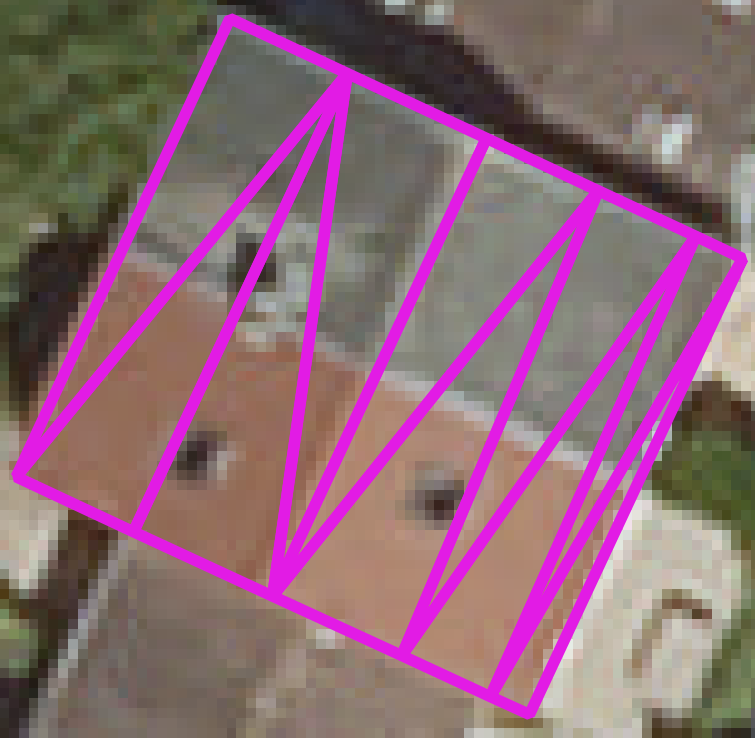
\includegraphics[height=.11\textheight]{images/Building_Errors/under_segmentation}}
                        \ffigbox[\FBwidth]{\caption{\textit{BOS}}\label{fig::over_bul}}{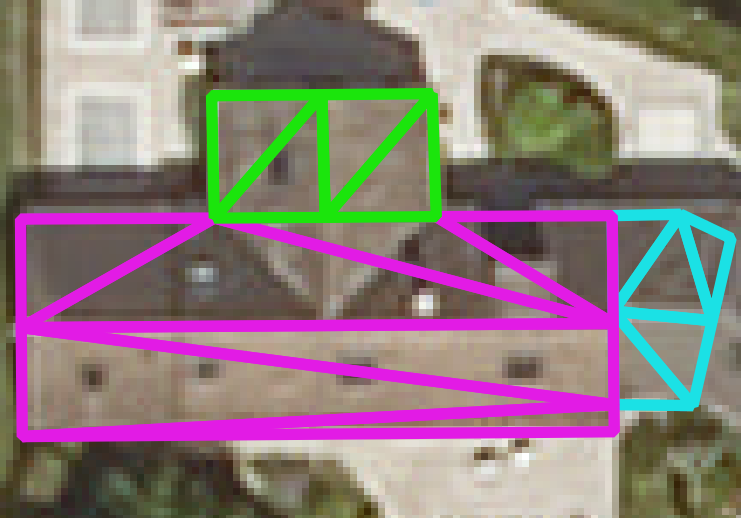
\includegraphics[height=.11\textheight]{images/Building_Errors/over_segmentation}}
                        \ffigbox[\FBwidth]{\caption{\textit{BInF}}\label{fig::footprint}}{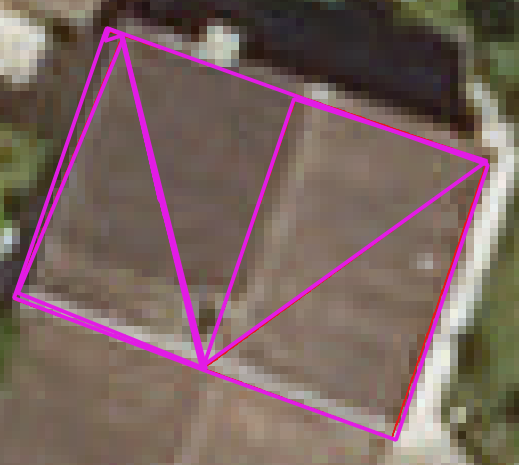
\includegraphics[height=.11\textheight]{images/Building_Errors/footprint}}
                        \ffigbox[\FBwidth]{\caption{\textit{BImH}}\label{fig::height}}{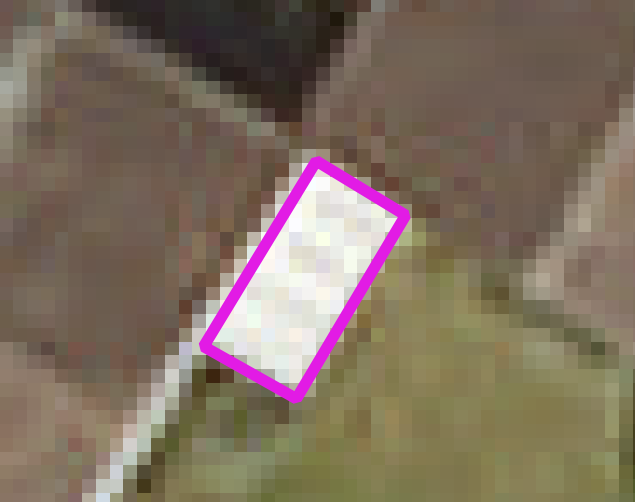
\includegraphics[height=.11\textheight]{images/Building_Errors/altimetric}}
                    \end{subfloatrow}
                }
                {
                    \captionsetup{labelfont={tiny, bf},textfont=scriptsize,justification=raggedright, labelsep=period}
                    \renewcommand{\thesubfigure}{\roman{SubFigCounter}}
					\vspace{-.3cm}
                    \captionof{subfigure}{Building errors family samples.}\label{fig::bul_err}
                    \refstepcounter{SubFigCounter}
                    \addtocounter{figure}{-1}
                }
                \ffigbox[\FBwidth]
                {
                    \begin{subfloatrow}[4]
                        \ffigbox[\FBwidth]{\caption{\textit{FUS}}\label{fig::under_fac}}{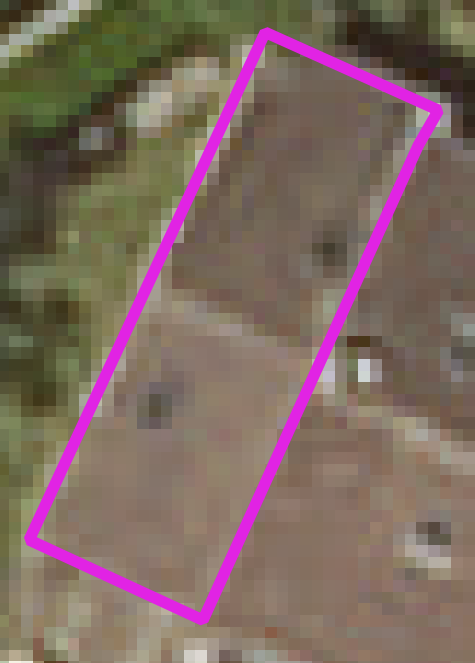
\includegraphics[height=.11\textheight]{images/Facet_Errors/under_segmentation}}
                        \ffigbox[\FBwidth]{\caption{\textit{FOS}}\label{fig::over_fac}}{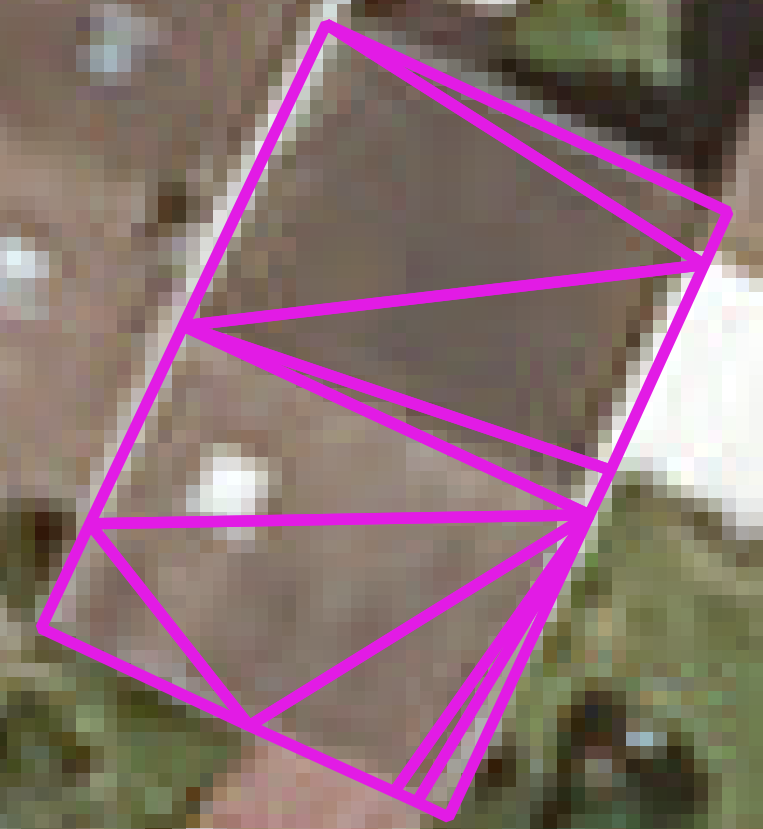
\includegraphics[height=.11\textheight]{images/Facet_Errors/over_segmentation}}
                        \ffigbox[\FBwidth]{\caption{\textit{FIS}}\label{fig::mis}}{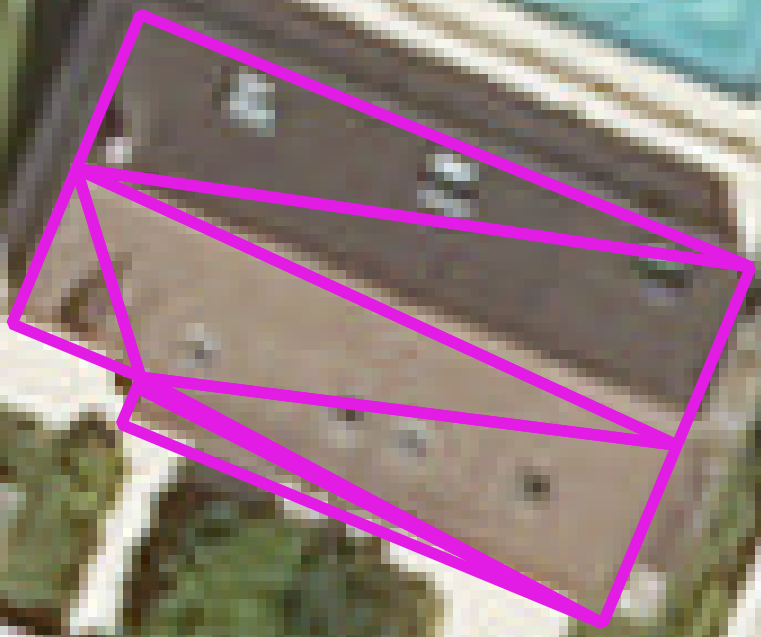
\includegraphics[height=.11\textheight]{images/Facet_Errors/mis_segmentation}}
                        \ffigbox[\FBwidth]{\caption{\textit{FImS}}\label{fig::slope}}{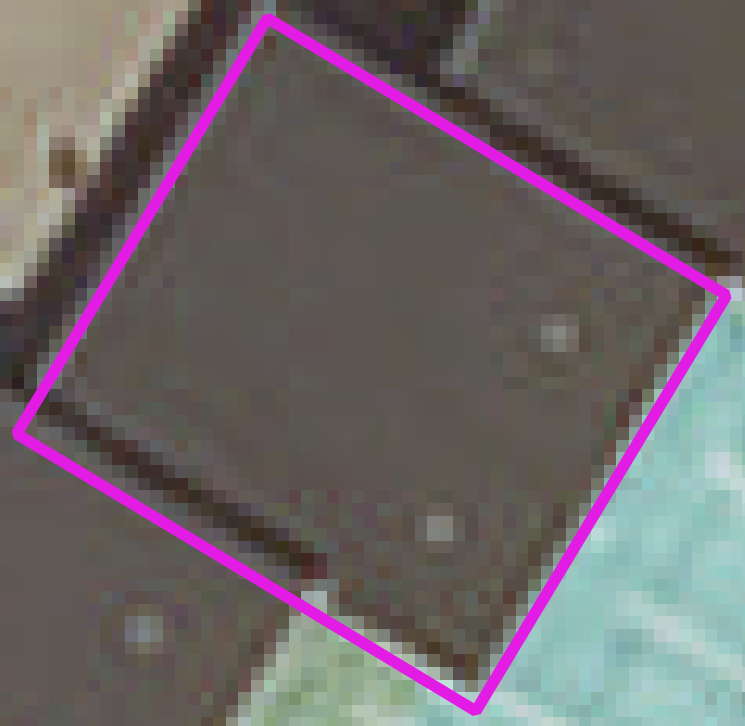
\includegraphics[height=.11\textheight]{images/Facet_Errors/slope}}
                    \end{subfloatrow}
                }
                {
                	\captionsetup{labelfont={bf},justification=raggedright, labelsep=period}
                    \renewcommand{\thesubfigure}{\roman{SubFigCounter}}
					\vspace{-.3cm}
                    \captionof{subfigure}{Facet errors family samples.}\label{fig::fac_err}
                    \refstepcounter{SubFigCounter}
                    \addtocounter{figure}{-1}
                }
            }
            {
            	\vspace{-.4cm}
                \caption{\label{fig::samples}Illustration of various errors of our taxonomy. One can see that geometric, spectral and height information are required for an accurate detection of all kinds of errors.}
            }
        \end{center}
    \end{figure*}

\subsection{Feature baseline}

	We propose a simple handcrafted set. We limit ourself to the validation of the semantic approach and taxonomy validation. We rely on three modalities. The first is the input 3D model. We extract statistics (maximum, minimum, mean, median and standard deviation) over attributes that describe the geometry of the building facets: number of nodes, area, angle between normals, distance between centroids and circumference. We add height attributes. These are represented by the histogram of the discrepancy between the rasterized model height map and the \acrshort{acr::dsm} at the same spatial resolution. It is chosen to be lower than building dimensions but higher than the modeling inherent planimetric uncertainty. Last comes optical features, computed by back-projecting the model on corresponding VHR orthoimage. For each facet edge, we compute a correlation histogram to image edges (cosine similarity between local gradients and the edge normal). This histogram is summed over all facet edges and then over all projected facets. Histograms concentrated near the value $1$ means facet edges correspond to genuine ones in the VHR image. Each modality provides 20 features.

\subsection{Classification process}

The labels are organized into different classification problems. To account for the desired modularity and flexibility, a random forest classifier is chosen (1,000 trees, maximal depth of 4). The depth is kept shallow in order to avoid overfitting while the large number of estimators deals with the large feature space variability. The \textit{Multi-label} setting is managed using a One vs All strategy on top of our classifier.

\section{Experiments}
\label{sec:expe}

We evaluate our approach on a dataset drawn from three French cities: Elancourt, Nantes and the XIII$^e$ arrondissement of Paris (Paris-13). Elancourt exhibits a high diversity of building types between residential districts with mostly bi-level buildings and  industrial areas with flat roofs. Nantes, in the other hand, represents a dense urban setting less diversified than the previous one. In Paris-13, high towers in the south coexist with Haussmann style buildings. Studied 3D models were obtained, using the algorithm described in~\cite{Durupt2006}, out of existing footprints and an aerial multi-view \acrshort{acr::dsm}. They were annotated according to the atomic errors list provided by our taxonomy. More details are reported in the table~\ref{tab::dataset}.

\begin{table}
	\begin{center}
		\scriptsize
        \begin{tabular}{c c c c}
            \toprule
            & Elancourt & Nantes & Paris-13 \\
            \midrule
            \# samples & 2009 & 748 & 478 \\
            \acrshort{acr::dsm} resolution & \SI{0.06}{\m} & \SI{0.1}{\m} & \SI{0.1}{\m} \\
            Orthoimage resolution & \SI{0.06}{\m} & \SI{0.1}{\m} & \SI{0.1}{\m} \\
            \bottomrule
        \end{tabular}
        \vspace{-.5cm}
        \caption{\label{tab::dataset} Dataset details.}
	\end{center}
\end{table}

Based on the devised pipeline, four feature configurations were tested: ``geometric features'' only, ``geometric and height features'', ``geometric and image features'' as well as ``geometric, height and image features''. A \SI{0.06}{\m}/\SI{0.10}{\m} spatial resolution \acrshort{acr::dsm} and integral orthorectified image are used to derive altimetric and optical features. Labels are extracted from a non \textbf{exclusive} and \textbf{\acrshort{acr::elod}} $=$ \acrshort{acr::lod}-$2$ taxonomy. We report here only the \textit{finesse} level of $3$. We perform a $10$-fold cross validation.
\begin{table*}
	\scriptsize
	\begin{center}
        \begin{tabular}{|x{1.4cm} | x{1.2cm} x{1.2cm} | x{1.2cm} x{1.2cm} | x{1.2cm} x{1.2cm} | x{1.2cm} x{1.2cm}|}
			\hline
            &\multicolumn{2}{x{2.4cm}|}{\textbf{Geometry}} & \multicolumn{2}{x{2.4cm}|}{\textbf{Geom. $\cup$ Height}} & \multicolumn{2}{x{2.4cm}|}{\textbf{Geom. $\cup$ Image}} & \multicolumn{2}{|x{2.4cm}|}{\textbf{All}}\\
            \cline{2-9}
            &\textbf{Recall} & \textbf{Prec.} & \textbf{Recall} & \textbf{Prec.} & \textbf{Recall} & \textbf{Prec.} & \textbf{Recall} & \textbf{Prec.}\\
            \hline
            \textit{BOS} & 93.96 & 76.15 &$93.36$ & \textbf{77.66} & 91.51 & 76.08 & 90.83 & 76.14 \\
            \hline
            \textit{BUS} & 32.98 & 76.47 &$31.52$ & \textbf{78.57} & 40.38 & 71.00 & 39.32 & 71.81 \\
            \hline
            \textit{BIB} & 12.32 & 67.57 & $22.34$ & $67.74$ & 16.26 & 67.35 & 16.75 & 68.0 \\
            \hline
            \textit{BIT} & 25.25 & 92.59 & $22.34$ & $67.74$ & 20.20 & 95.24 & 11.11 & 91.67 \\
            \hline
            \hline
            \textit{FOS} & 98.91 & 99.07 & \textbf{98.87} & $98.67$ & 98.99 & 98.84 & 98.91 & 98.84 \\
            \hline
            \textit{FUS} & 1.90 & 54.55 &$0.70$ & $33.34$ & 1.61 & 50 & 1.27 & 66.67 \\
            \hline
            \textit{FIB} & 9.17 & 87.5 &$1.36$ & $50.00$ & 8.30 & 82.61 & 7.42 & 100 \\
            \hline
            \textit{FIT} & 6.67 & 100 &$1.36$ & $50.00$ & 3.33 & 100 & 3.33 & 100 \\
            \hline
            \textit{FIG} & 80.54 & 73.14 & $0$ & --- & 78.69 & 72.12 & 79.02 & 71.82 \\
            \hline
		\end{tabular}
	\end{center}
    \vspace{-.5cm}
    \caption{\label{tab::ablation}Results (\%) for the \textit{finesse} level $3$. All \textit{atomic} errors are considered over all possible configurations.}
\end{table*}

\begin{table*}
	\begin{center}
    	\scriptsize
		\begin{tabular}{|x{1cm} | x{1.3cm} x{1.3cm} | x{1.2cm} x{1.2cm} | x{1.2cm} x{1.2cm}| x{1.2cm} x{1.2cm}|}
            \hline
            & \multicolumn{2}{x{2.4cm}|}{\textbf{Elancourt $\rightarrow$ Nantes}} & \multicolumn{2}{x{2.5cm}|}{\textbf{Elancourt $\rightarrow$ Paris-13}} & \multicolumn{2}{x{2.5cm}|}{\textbf{Nantes $\rightarrow$ Elancourt}} & \multicolumn{2}{x{2.5cm}|}{\textbf{Paris-13 $\rightarrow$ Elancourt}}\\
            \cline{2-9}
            &\textbf{Recall} & \textbf{Prec.} & \textbf{Recall} & \textbf{Prec.} & \textbf{Recall} & \textbf{Prec.} & \textbf{Recall} & \textbf{Prec.} \\
            \hline
            \textit{BOS} & 93.12 & 42.61 & 96.53 & 43.82 & 86.47 & 64.99 & 82.14 & 69.59 \\
            \hline
            \textit{BUS} & 8.82 & 66.67 & 0 & --- & 23.75 & 57.47 & 25.0 & 50.49 \\
            \hline
            \textit{BImB} & 2.02 & 33.33 & 0 & --- & 15.65 & 46.75 & 19.89 & 48.05 \\
            \hline
            \textit{BInT} & 0.88 & 100 & 3.95 & 50.0 & 4.70 & 100 & 4.44 & 100 \\
            \hline
            \hline
            \textit{FOS} & 98.33 & 97.92 & 97.19 & 97.58 & 98.76 & 98.92 & 99.06 & 97.14 \\
            \hline
            \textit{FUS} & 13.81 & 63.04 & 8.36 & 95.83 & 1.68 & 77.78 & 3.53 & 89.47 \\
            \hline
            \textit{FIB} & 46.34 & 65.52 & 11.80 & 60.71 & 23.75 & 73.96 & 21.86 & 70.11 \\
            \hline
            \textit{FIT} & 9.09 & 100 & 0 & 0 & 3.57 & 100 & 4.34 & 33.33 \\
            \hline
            \textit{FIG} & 94.17 & 70.70 & 86.16 & 88.47 & 86.35 & 67.97 & 82.38 & 73.08 \\
            \hline
        \end{tabular}
        \caption{\label{tab::transferability} Transferabilty study on different urban scene.}
	\end{center}
\end{table*}

Discussion results.

Qualitative assessment is also performed in order to illustrate some failure cases (Figure~\ref{fig::results}, from left to right). In the first image, the similarity of the building outline to over segmented buildings cases induces an overdetection. In the second example, the building is wrongfully detected as being under segmented due to the presence of a balcony and a smaller annex building. In the third building, while correctly predicting \textit{BOS}, our algorithm fails to detect the under segmented roof. Finally, in the last depiction, except the well caught footprint error, defects are overlooked as there are few comparable samples in the dataset. To alleviate these issues, more robust features could be introduced taking into account higher order information. Dataset enrichment could be another option which provides more instances of underrepresented errors. In the end, we can also add the human in the loop through manual interactive evaluation which can adapt well to user-specific needs.

\begin{figure*}
	\begin{center}
    \tiny
		\begin{tabular}{| x{1.11cm} | x{.75cm} | x{.75cm} || x{1.11cm} | x{.75cm} | x{.75cm} || x{1.11cm} | x{.75cm} | x{.75cm} || x{1.11cm} | x{.75cm} | x{.75cm} |}
			\hline
			\multicolumn{3}{| c ||}{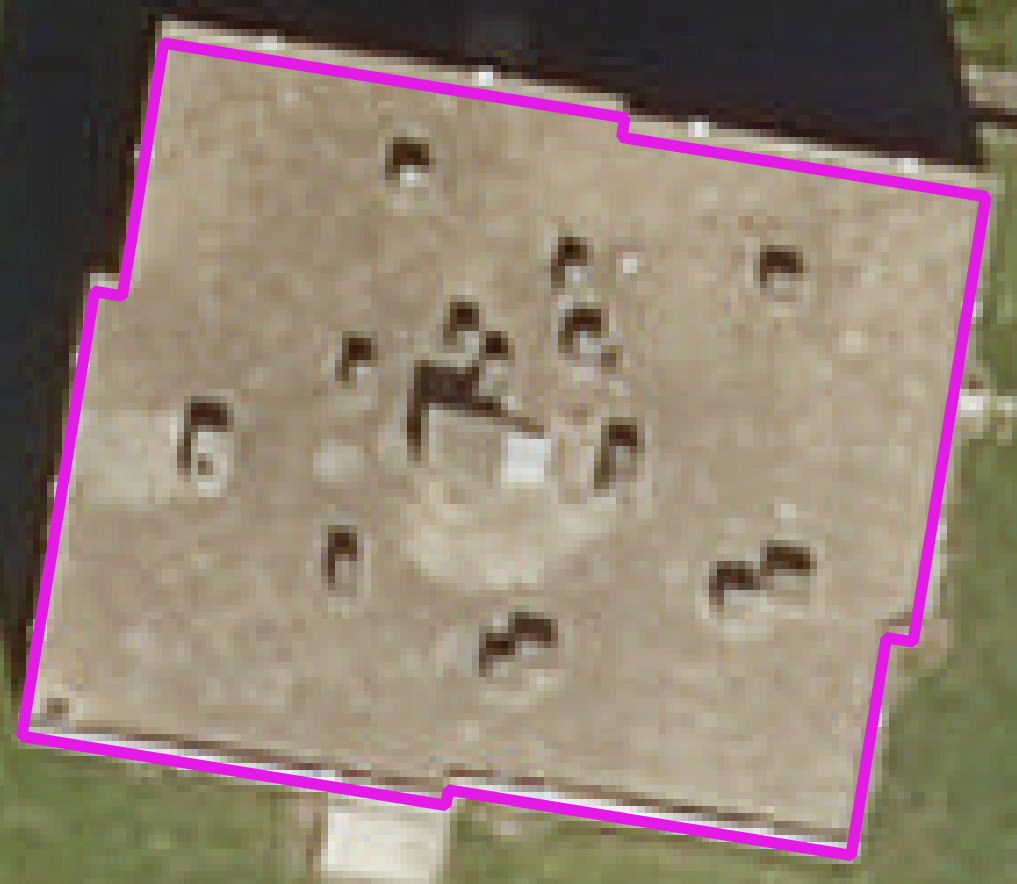
\includegraphics[height=.1\textheight,valign=m,margin=.1cm .1cm]{images/prediction_results/valid_as_bul_over}} & \multicolumn{3}{ c ||}{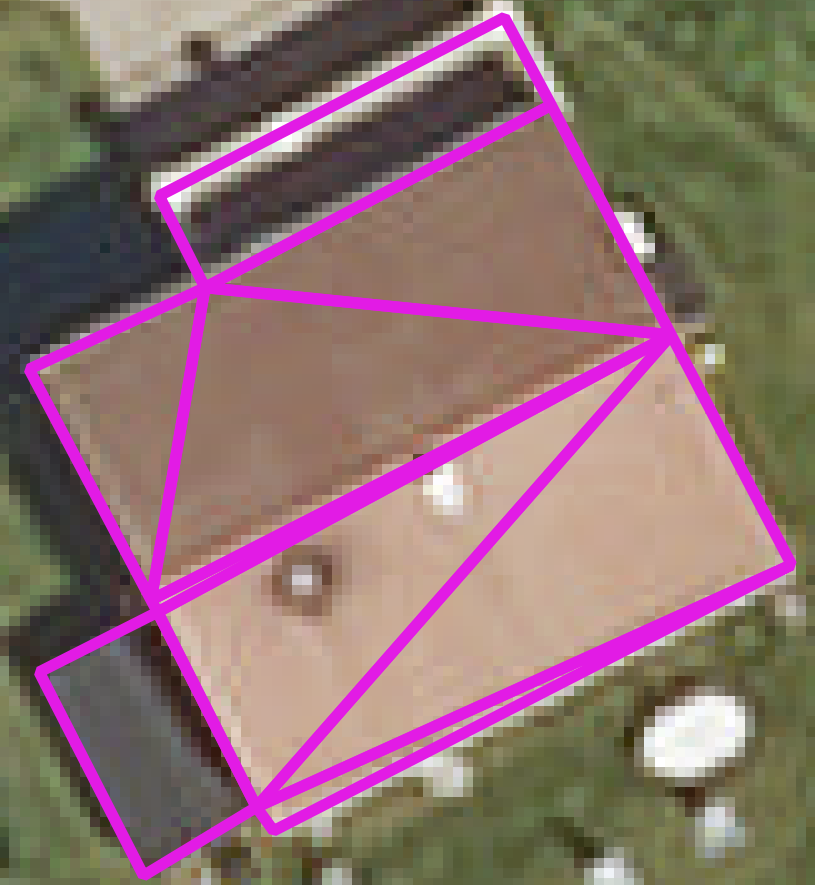
\includegraphics[height=.1\textheight,valign=m,margin=0cm .1cm]{images/prediction_results/no_imprec_no_fac_over}} & \multicolumn{3}{ c ||}{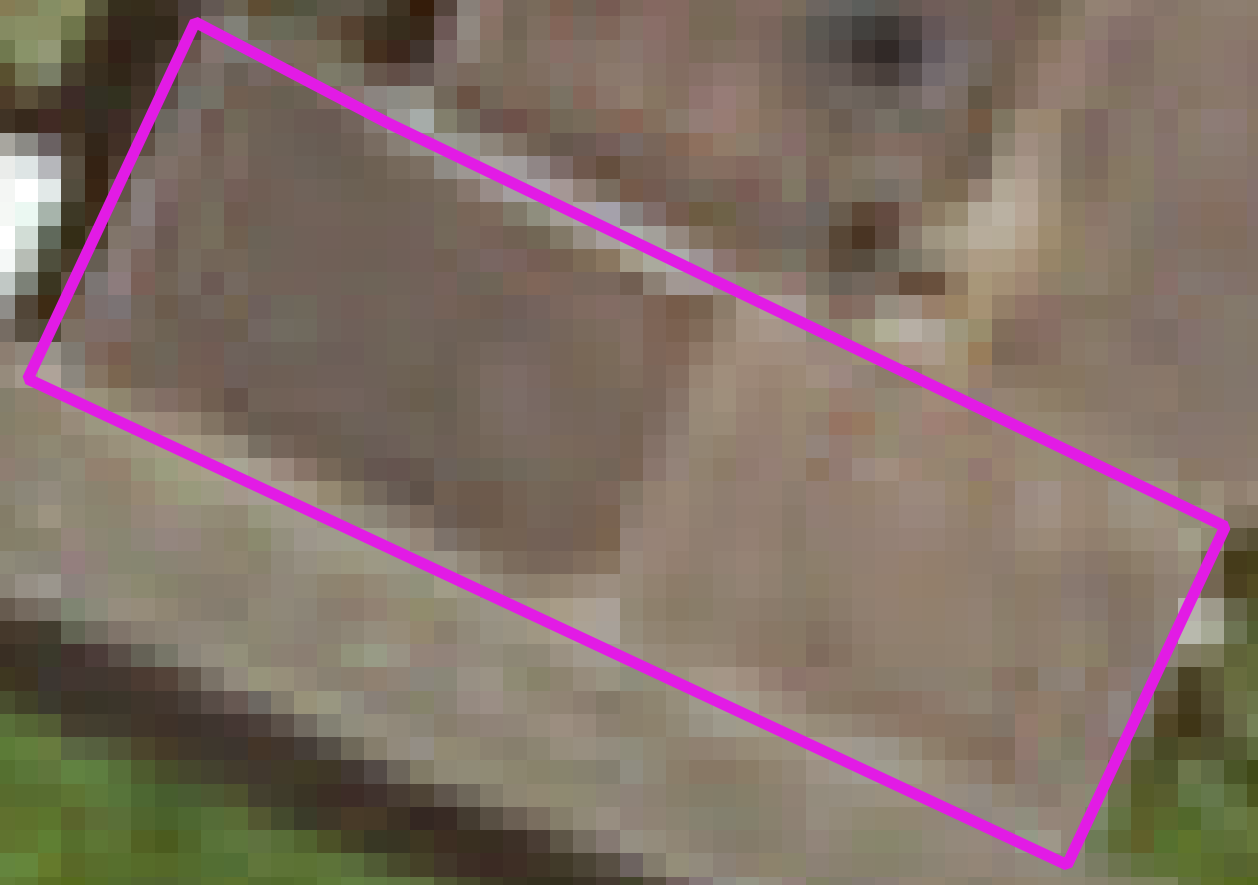
\includegraphics[height=.1\textheight,valign=m,margin=0cm .1cm]{images/prediction_results/no_under_seg}} & \multicolumn{3}{ c |}{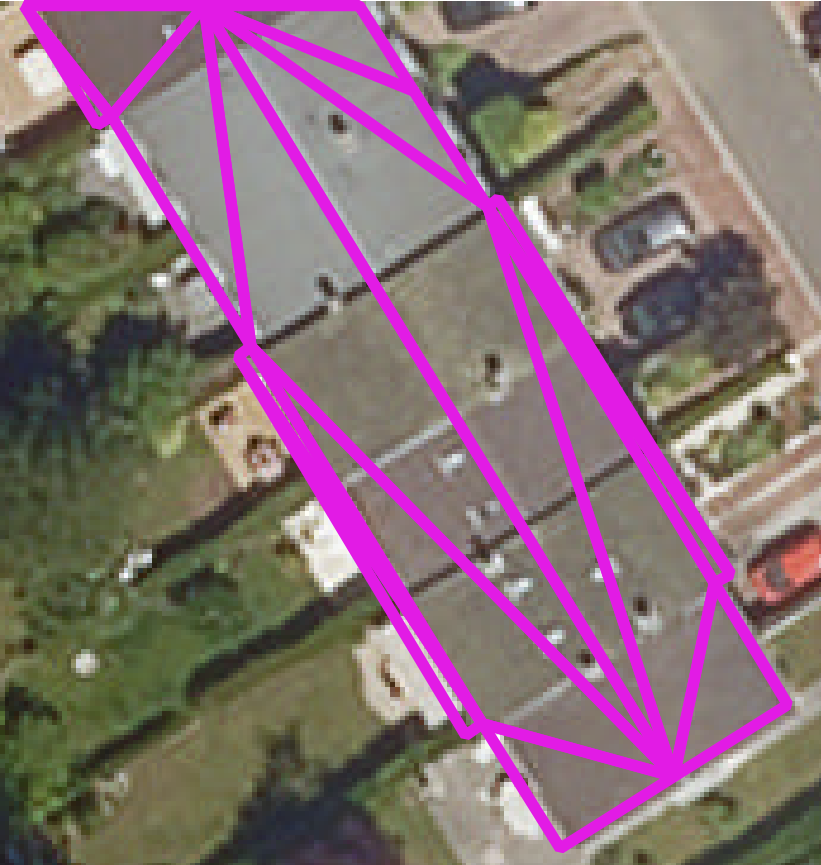
\includegraphics[height=.1\textheight,valign=m,margin=0cm .1cm]{images/prediction_results/no_bul_under_seg}} \\
			\hline
			\textbf{Errors} & \textbf{G.T.} & \textbf{Pred.} & \textbf{Errors} & \textbf{G.T.} & \textbf{Pred.} & \textbf{Errors} & \textbf{G.T.} & \textbf{Pred.} & \textbf{Errors} & \textbf{G.T.} & \textbf{Pred.}\\
            \hline
            \textit{BOS} & \xmark & \cmark & \textit{BUS} & \xmark & \cmark & \textit{BOS} & \cmark & \cmark & \textit{BOS} & \cmark & \xmark \\
            Valid & \cmark & \xmark & \textit{FImS} & \cmark & \xmark & \textit{FUS} & \cmark & \xmark &  \textit{FOS} & \cmark & \xmark \\
             &  &  & \textit{FOS} & \cmark & \xmark &  &  &  & \textit{BUS} & \cmark & \xmark \\
             &  &  &  &  &  &  &  &  &  \textit{BInF} & \cmark & \cmark \\
            \hline
		\end{tabular}
        \vspace{-.5cm}
        \caption{\label{fig::results} Predicted (Pred.) errors compared to ground truth (G.T.) labels are illustrated in some pathological cases. Knowing how each error is represented in the dataset helps interpreting mispredictions.}
	\end{center}
\end{figure*}

\section{Conclusion}
\label{sec::conclusion}

We proposed a framework to semantically evaluate 3D building models. Errors were hierarchically organized into a flexible and parametrized taxonomy, handling the large diversity of urban environments and end users' requirements. Model quality was predicted using a supervised classifier using three modalities. Although being mitigated over under-represented errors, results are satisfactory in the well balanced cases. As a next step, more structurally aware features (e.g., based on graph comparison) will be proposed, so as to be applied on a richer and more diverse dataset (potentially involving data augmentation) under a deep-based framework.

\bibliographystyle{IEEEtran}
\bibliography{IEEEabrv,references}
\end{document}
